\begin{figure}[t!]
    \setlength{\belowcaptionskip}{-1em}
    \centering

    % \subfloat[][Using \tool for debugging.]{
        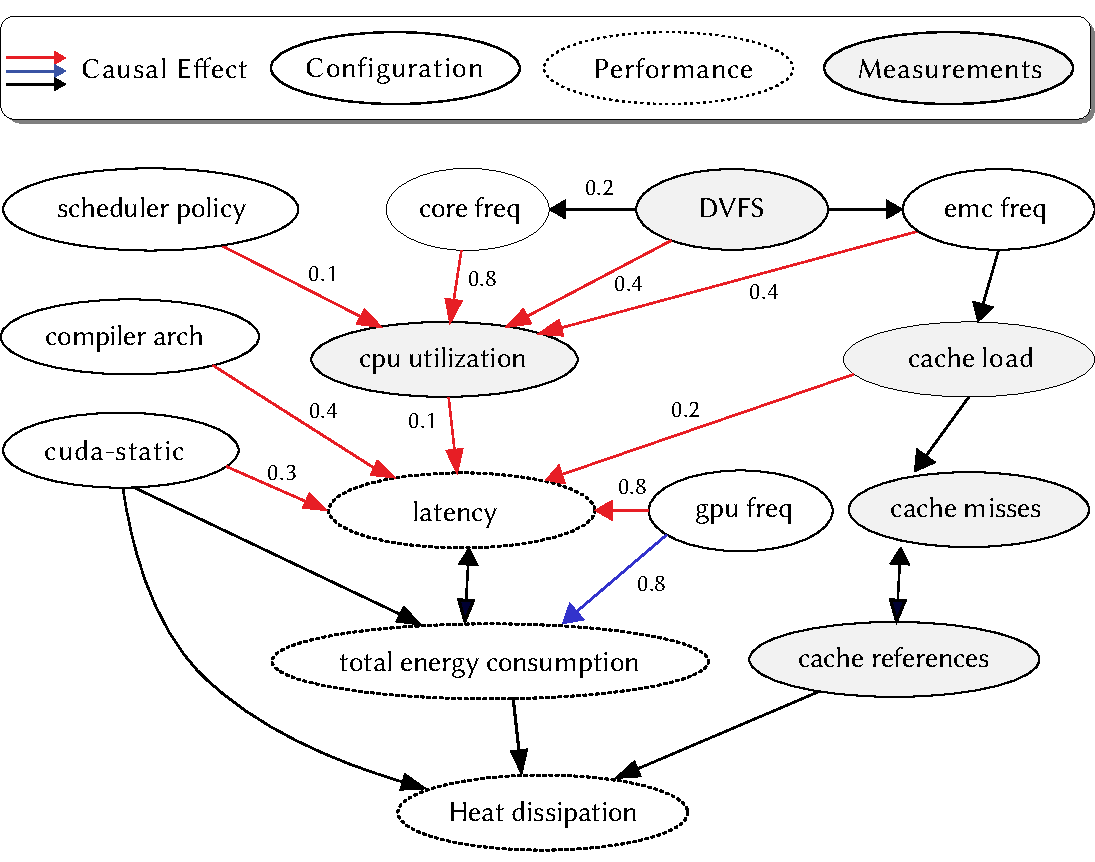
\includegraphics[width=\linewidth]{fig__cauper_samp.pdf}\label{fig:cauper_samp}
        % }
    %
    %
    %
    % \subfloat[][Using \texttt{iperf} and \texttt{top} command line profilers for debugging.]{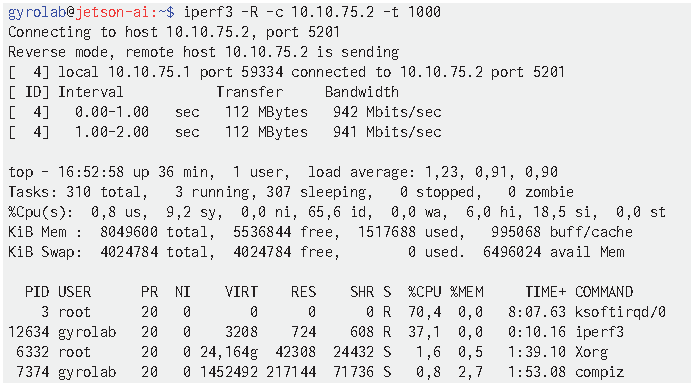
\includegraphics[width=0.5\linewidth]{fig__iperf.pdf}\label{fig:iperf_samp}}
    
    \caption{\small A simplified causal model used in \tool. \protect\edgeone~shows the causal paths between configurations and between configurations and non-functional properties like latency, energy consumption, \etc. The numbers represent the magnitude of causal effect.}
    % \caption{\small Mechanisms to debug non-functional faults. Here, (a) shows a simplified causal model \tool builds to debug non-functional faults, \eg, when debugging for latency, the \red{$\boldsymbol{\longrightarrow}$} shows the causal paths from the configurations to latency and the numbers represent the magnitude of causal effect; (b) shows an sample \texttt{iperf} (for network load information) and \texttt{top} (for system load information) trace used to pinpoint and fix a real-world performance bug~\cite{HighCPUu7:online}}
    \label{fig:sample}
\end{figure}